\documentclass[lecture,12pt,]{pcms-l}
\input preamble.tex

% For faster processing, load Matlab syntax for listings
\definecolor{MyDarkGreen}{rgb}{0.0,0.4,0.0}
\lstloadlanguages{Matlab}%
\lstset{language=Matlab,
        frame=single,
        basicstyle=\small\ttfamily,
        keywordstyle=[1]\color{Blue}\bf,
        keywordstyle=[2]\color{Purple},
        keywordstyle=[3]\color{Blue}\underbar,
        identifierstyle=,
        commentstyle=\usefont{T1}{pcr}{m}{sl}\color{MyDarkGreen}\small,
        stringstyle=\color{Purple},
        showstringspaces=false,
        tabsize=5,
        % Put standard MATLAB functions not included in the default
        % language here
        morekeywords={xlim,ylim,var,alpha,factorial,poissrnd,normpdf,normcdf},
        % Put MATLAB function parameters here
        morekeywords=[2]{on, off, interp},
        % Put user defined functions here
        morekeywords=[3]{FindESS},
        morecomment=[l][\color{Blue}]{...},
        numbers=left,
        firstnumber=1,
        numberstyle=\tiny\color{Blue},
        stepnumber=0
        }

% Only the next five fields need to be edited.
\newcommand{\lecAuth}{William M. McEneaney}
\newcommand{\scribe}{Thomas Denewiler, Gideon Prior}
\newcommand{\authEmail}{wmceneaney@ucsd.edu}
\newcommand{\scribeEmail}{tdenewiler@gmail.com}
\newcommand{\course}{MAE 288A: Optimal Control}
\newcommand{\lectureNum}{4}

\address{Department of Mechanical and Aerospace Engineering, University of California, San Diego}

% Adds a hyperlink to an email address.
\newcommand{\mailto}[2]{\href{mailto:#1}{#2}}

% These commands set the document properties for the PDF output. Needs the hyperref package.
\hypersetup
{
    colorlinks,
    linkcolor={black},
    citecolor={black},
    filecolor={black},
    urlcolor={black},
    pdfauthor={\scribe <\mailto{\scribeEmail}{\scribeEmail}>},
    pdfsubject={\course},
    pdftitle={Lecture \lectureNum},
    pdfkeywords={UC San Diego, Optimal Control},
    pdfstartpage={1},
}

% Includes a figure
% The first parameter is the label, which is also the name of the figure
%   with or without the extension (e.g., .eps, .fig, .png, .gif, etc.)
%   IF NO EXTENSION IS GIVEN, LaTeX will look for the most appropriate one.
%   This means that if a DVI (or PS) is being produced, it will look for
%   an eps. If a PDF is being produced, it will look for nearly anything
%   else (gif, jpg, png, et cetera). Because of this, when I generate figures
%   I typically generate an eps and a png to allow me the most flexibility
%   when rendering my document.
% The second parameter is the width of the figure normalized to column width
%   (e.g. 0.5 for half a column, 0.75 for 75% of the column)
% The third parameter is the caption.
\newcommand{\scalefig}[3]{
  \begin{figure}[ht!]
    % Requires \usepackage{graphicx}
    \centering
	\fbox{
	    \includegraphics[width=#2\columnwidth]{#1}
	}
    %%% I think \captionwidth (see above) can go away as long as
    %%% \centering is above
    %\captionwidth{#2\columnwidth}%
    \caption{#3}
    \label{#1}
  \end{figure}}

% Includes a MATLAB script.
% The first parameter is the label, which also is the name of the script
%   without the .m.
% The second parameter is the optional caption.
\newcommand{\matlabscript}[2]
  {\begin{itemize}\item[]\lstinputlisting[caption=#2,label=#1]{#1.m}\end{itemize}}

% Example environment.
\newtheoremstyle{example}{\topsep}{\topsep}	%
     {}%         Body font
     {}%         Indent amount (empty = no indent, \parindent = para indent)
     {\bfseries}% Thm head font
     {}%        Punctuation after thm head
     {\newline}%     Space after thm head (\newline = linebreak)
     {\thmname{#1}\thmnumber{ #2}\thmnote{ #3}}%         Thm head spec

   \theoremstyle{example}
   \newtheorem{example}{Example}[section]

% A command to show a vector norm that will have the pipe signs scale with the contents.
\newcommand{\vectornorm}[1]{\left|\left|#1\right|\right|}
\newcommand{\SI}{System Identification}


%%%%%%%%%%%%%%%%%%%%%%%%%%%%%%%%%%%%%%%%%%%%%%%%%%%%%%%%%%%%%


\begin{document}
\mainmatter
\setcounter{page}{1}

\lectureseries[\course]{\course}

\auth[\lecAuth]{Lecturer: \lecAuth\\ Scribe: \scribe}
\date{October 8, 2009}

\setaddress

% the following hack starts the lecture numbering at 4
\setcounter{lecture}{3}
\setcounter{chapter}{3}

\lecture{Dynamic Programming}

\section{System Basics}
Recall that the dynamics and initial conidtions of the system are given by
\begin{align*}
\xi_{t+1} &= f(\xi_t,u_t,w_t) \\
\xi_0 &= x
\end{align*}
The cost function is
$$J(s,x,w) = E[\sum_{t=s}^{T-1}l(\xi_t,u_t) + \phi(\xi_t)]$$
with $u_t=w_t(\xi_t)$. The value function is given by
$$V(\Delta,x) = \inf_{w\in M_{s,T-1}} j(s,x,w)$$
Also,
$$\tilde{M}_{\tau_1,\tau_2} = \{\{w_r\}_{r=\tau_1}^{\tau_2} | w_r:\{\xi_r\}_{r=\tau_1}^{\tau_2}\} \to u\in\mathcal{U}$$
This holds $\forall r\in\tau_1,\ldots,\tau_2 \text{ s.t. } \forall t\in\tau_1,\ldots,\tau_2, ~\forall \xi, ~\forall \eta$. Then,
$$w_r(\xi_\tau,\xi_{\tau+1},\ldots,\xi_t,\eta_t,\eta_{t-1},\ldots,\eta_{\tau_2}) = w_r(\xi_{\tau_1},\xi_{\tau_1+1},\xi_{\tau_2})$$
These are non-anticipative controls and are known as dynamic programming (DP).

\section{Infinum}
Let $A\subseteq\mathbb{R}$ and $\min A$ is the smallest element of $A$.

\begin{example}
\begin{align*}
&\min([2.7,\pi)) = 2.7 \\
&\min((2.7,\pi)) \text{ DNE}
\end{align*}
where DNE means ``does not exist''.
\end{example}
$\lozenge$

\begin{definition}
Infinum $\doteq$ the greatest lower bound.
\end{definition}

$z = \inf A$ iff $y\leq z$ $\forall x\in A$ and $y>z\to\exists x\in A: y>x$. In english this means
\begin{itemize}
\item The infinum is smaller than anything in $A$.
\item Add anything to the infinum and there is something in $A$ larger than it.
\end{itemize}
$\inf A = \min A$ if $\min A$ exists. And yet
\begin{align*}
\inf((2.7,\pi)) &= 2.7 \\
\inf\left(\left\lbrace\frac{1}{n}\right\rbrace_{N=1}^\infty\right) &= 0
\end{align*}
Note the the supremum is the opposite, or the least upper bound.

\begin{example}
\begin{align*}
\xi_t &= N_t \\
\xi_0 &= 0 \\
U_t&\in\{-1,1\}
\end{align*}
The last expression means that $U_t$ is either $1$ or $-1$ and is not convex. Minimize
$$\int_0^T|\xi_t|^2 + |u_t|^2dt = \int_0^T|\xi_t|^2 + 1dt$$
See Figure \ref{fig:04signal} to see $u_t$. This leads to
\begin{align*}
|\xi_t| &\leq \frac{T}{2N} ~\forall t \\
\Rightarrow \int_0^T|\xi_t|^2+|u_t|^2dt &\leq \int_0^t\frac{T^2}{(2N)^2} + 1 \to 1 \text{ as } N\to\infty
\end{align*}
Therefore, the infinum of $\int_0^T|\xi_t|^2+|N_t|^2dt = 1$ but its minimum does not exist.
\end{example}
$\lozenge$

\begin{figure}[ht!]
	\centering
	\includegraphics[width=.4\textwidth]{images/04signal}
	\caption{Original signal in red and integrated signal in blue.}
	\label{fig:04signal}
\end{figure}

\section{Dynamic Programming}
What is the cheapest flight from San Diego to Boston with two stops or less when the allowable cities for stops are San Diego, Los Angeles, Chicago, Atlanta, New York City and Boston? The state space is
$$\{\text{San Diego, Los Angeles, Chicago, Atlanta, New York City, Boston}\}$$
Each flight from one city to a different city has a cost. Let $C(x,y)$ be the cost from city $x$ to city $y$.

\subsection{Dynamic Programming Principle}
$$\min C\{\text{SAN, BOS}\} = \min\{C(SAN,x) + \min(\text{1 stop cost from }x\to\text{BOS}\}$$
Let $V(t,x) =$ min cost from $x$ at stop $t$ to Boston.
\begin{align*}
V(3,x) &= \begin{cases} 0, & x=\text{BOS} \\ \infty, & x\neq\text{BOS} \end{cases} \\
V(2,x) &= C(x,\text{BOS}) \\
V(1,x) &= \min[C(x,y)+V(2,y)] \\
V(0,x) &= \min[C(x,y)+V(1,y)]
\end{align*}
Recall that $\xi_{t+1}=f(\xi_t,w_t)$ where we are ignoring control for the moment. The conditional expectation is then
$$E[\{\xi_{t+1},\xi_{t+2},\ldots,\xi_T\}|\xi_t=y] = E[f(y,f(y,w_t)),f(f(y,w_t),w_{t+1}),\ldots]$$
This represents integration over the $w$'s.
\begin{align*}
&\int_{w_{T-1}}\cdots\int_{w_{t+1}}\int_{w_t}f(y,f(y,w_t)),f(f(y,w_t),w_{t+1}),\ldots,f(f(y,w_t),w_{T-1})dw_t\cdots dw_{T-1} \\
= &\int\cdots\int P_{w_t}(w_t)\cdots P_{w_{t-1}}(w_{t-1})dw_t\cdots dw_{T-1}
\end{align*}

\begin{theorem}{Dynamic Programming Principle}
Let $t\in~]s,T-1[$. Then
\begin{align}
\label{eq:dpp}
V(s,x) = \inf_{\mu\in\mathcal{M}_{]s,t-1[}}E\left\lbrace\sum_{r=s}^{t-1}l(\xi_r,w_r(\xi)) + V(t,\xi_t)\right\rbrace
\end{align}
The expectation taken over $w_s,\ldots,w_{t-1} = w_{]s,t-1[}$.
\end{theorem}

\begin{proof}
The notation $]a,b[$ operator means greater than $a$ and less than $b$. Let $R(s,x) = $ right hand side of (\ref{eq:dpp}). For any $y\in\mathbb{R}^N$, by definition the value $V(t,y) = \inf_{\mu\in\mathcal{M}]t,T-1[}$. This gives
$$E_{w_{]t,T-1[}}\left\lbrace \sum_{r=k}^{T-1}l(\xi_r,\mu_r(\xi))+\phi(\xi_T)\right\rbrace$$
Introduce the notation $x$ is $\Sigma$-optimal for $\inf A$ if $x\in A, x\leq\inf A+\Sigma$. Let $\mu^{\Sigma,y}\in\tilde{M}_{]t,T-1[}$ be $\Sigma$-optimal, then
\begin{align}
\label{eq:dppvalue}
V(t,y) + \Sigma\geq E_{w_{]t,T-1[}}\left\lbrace \sum_{r=t}^{T-1}l(\xi_r^{\Sigma,y}, \mu_r^{\Sigma,y}(\xi^{\Sigma,y}) + \phi(\xi_T^{\Sigma,y})\right\rbrace
\end{align}
with $\xi^{\Sigma,y}$ satisfying the dynamics and $\xi_t^{\Sigma,y} = y$ and control $\mu^{\Sigma,y}$. Substitute (\ref{eq:dppvalue}) into (\ref{eq:dpp}), then
\begin{align*}
R(s,x) \geq &\inf_{w\in\tilde{\mathcal{M}}_{]s,t-1[}} E_{w_{]s,t-1[}}\left\lbrace \sum_{r=s}^{T-1}l(\xi_r,w_r(\xi))\right\rbrace \\
&+ E\left\lbrace \sum_{r=t}^{T-1}l(\xi^{\Sigma,y},w^{\Sigma,y}(\xi^{\Sigma,y})\right\rbrace + \phi(\xi_T^{\Sigma,y}) - \Sigma
\end{align*}
Let
$$\tilde{\mu}(\xi) = \begin{cases} \bar{w}_2(\xi_{]s,t-1[}, & r\leq t-1 \\ w_r^{\Sigma,\xi_\tau}(\xi_{]t,T-1[}), & r\geq t \end{cases}$$
\textit{Exercise:} Show $\tilde{\mu}\in\tilde{\mathcal{M}}_{]s,T-1[}$.

Then we have
$$R(s,x) \geq \cdots = E_{\mu_{]s,T-1[}}\left\lbrace\sum_{r=s}^{T-1} l(\tilde{\xi}_r,\tilde{w}_r(\tilde{\xi})) + \phi(\tilde{\xi}_r)\right\rbrace - 2\Sigma$$
where $\tilde{\xi}$ satisfies the dynamics, $\tilde{\xi}_s=x$, and is driven by $\tilde{\mu}$. This leads to
$$R(s,x) \geq J(s,x,\tilde{w}) - 2\Sigma \geq V(s,x)-2\Sigma$$.
This is true $\forall \Sigma>0\to R(s,x)\geq V(s,x)$. Note that if $A\geq B-\Sigma ~\forall \Sigma > 0$, $A,B$ independent of $\Sigma$, then $A\geq B$. This proof can be finished as an exercise.
\end{proof}

DPP is ``universally'' true. This needs to be shown for particular problem classes.

\begin{example}
One step forward in time.
\begin{align}
\label{eq:dpe}
t &= s+1 \nonumber \\
V(s,x) &= \inf_{w\in\tilde{\mathcal{M}}} E_{w_s}\left\lbrace l(\xi_s,w_s(\xi_s)) + V(s+1,\xi_{s+1})\right\rbrace \nonumber \\
&= \inf_{w\in\tilde{\mathcal{M}}_{s,s}} \left\lbrace l(x,w_s(x)) + E_{w_s}[V(s+1,f(x,w_s(x),w_s)]\right\rbrace \nonumber \\
&= \inf_{u\in\mathcal{V}} \left\lbrace l(x,u) + E[V(s+1,f(x,u,w_s))]\right\rbrace \nonumber \\
&\text{in integral form} \nonumber \\
V(s,x) &= \inf_{u\in U} \left\lbrace l(x,u) + \int_{\mathbb{R}}V(s+1)f(x,u,w))P_{w_s}(w)dw\right\rbrace
\end{align}
Equation (\ref{eq:dpe}) is known as the Dynamic Programming Equation (DPE). For the third equality we used the definition $\xi_s \doteq x$.
\end{example}
$\lozenge$

\section{Backward DP}
\begin{align*}
V(T,x) &= \phi(x) \\
V(T-1,x) &= \inf_{u\in\mathcal{U}} \left\lbrace l(x,u) + E_{w_r}[V(T,f(x,u,w_s))]\right\rbrace \\
V(T-1,x) &= \cdots \\
&\vdots \\
&= V(s,x)
\end{align*}

This gives the optimal control (if minimizer exists) as
$$\mu_s \in \arg\min_{u} \left\lbrace l(x,u) + E[u(s+1,f(x,u,w_s))]\right\rbrace = \bar{\mu}_s(x)$$
Thus, we can see that optimal control is indeed a feedback on the current state.


\end{document}

%%%%%%%%%%%%%%%%%%%%%%%%%%%%%%%%%%%%%%%%%%%%%%%%%%%%%%%%%%%%%